\documentclass[12pt,a4paper]{article}
\usepackage[utf8]{inputenc}
\usepackage[spanish]{babel}
\usepackage[margin=0.5in, top=0.5in, bottom=0.5in]{geometry}
\usepackage{amsmath}
\usepackage{amsfonts}
\usepackage{amssymb}
\usepackage{hyperref}
\usepackage{graphicx}
\usepackage[shortlabels]{enumitem}
\newcommand{\p}{\phantom{......}}

\title{Bases de datos 2023-1\\
Práctica 1: Bitácora}
\begin{document}
\maketitle

\textbf{Reporte de instalación:}\\
\begin{enumerate}
    \item \textit{Sistema operativo y versión:} GNU\\linux 5.15.47-generic \\

    \item \textit{Distribución:} Ubuntu 22.04\\

    \item \textit{Versión de la instalación:} psql (PostgreSQL) 14.5\\

    \item \textit{Tiempo requerido:} 20min ()\\

    \item \textit{Paso a Paso:}\\
    
        Primero, instalo wget y ca-certificates: \\
        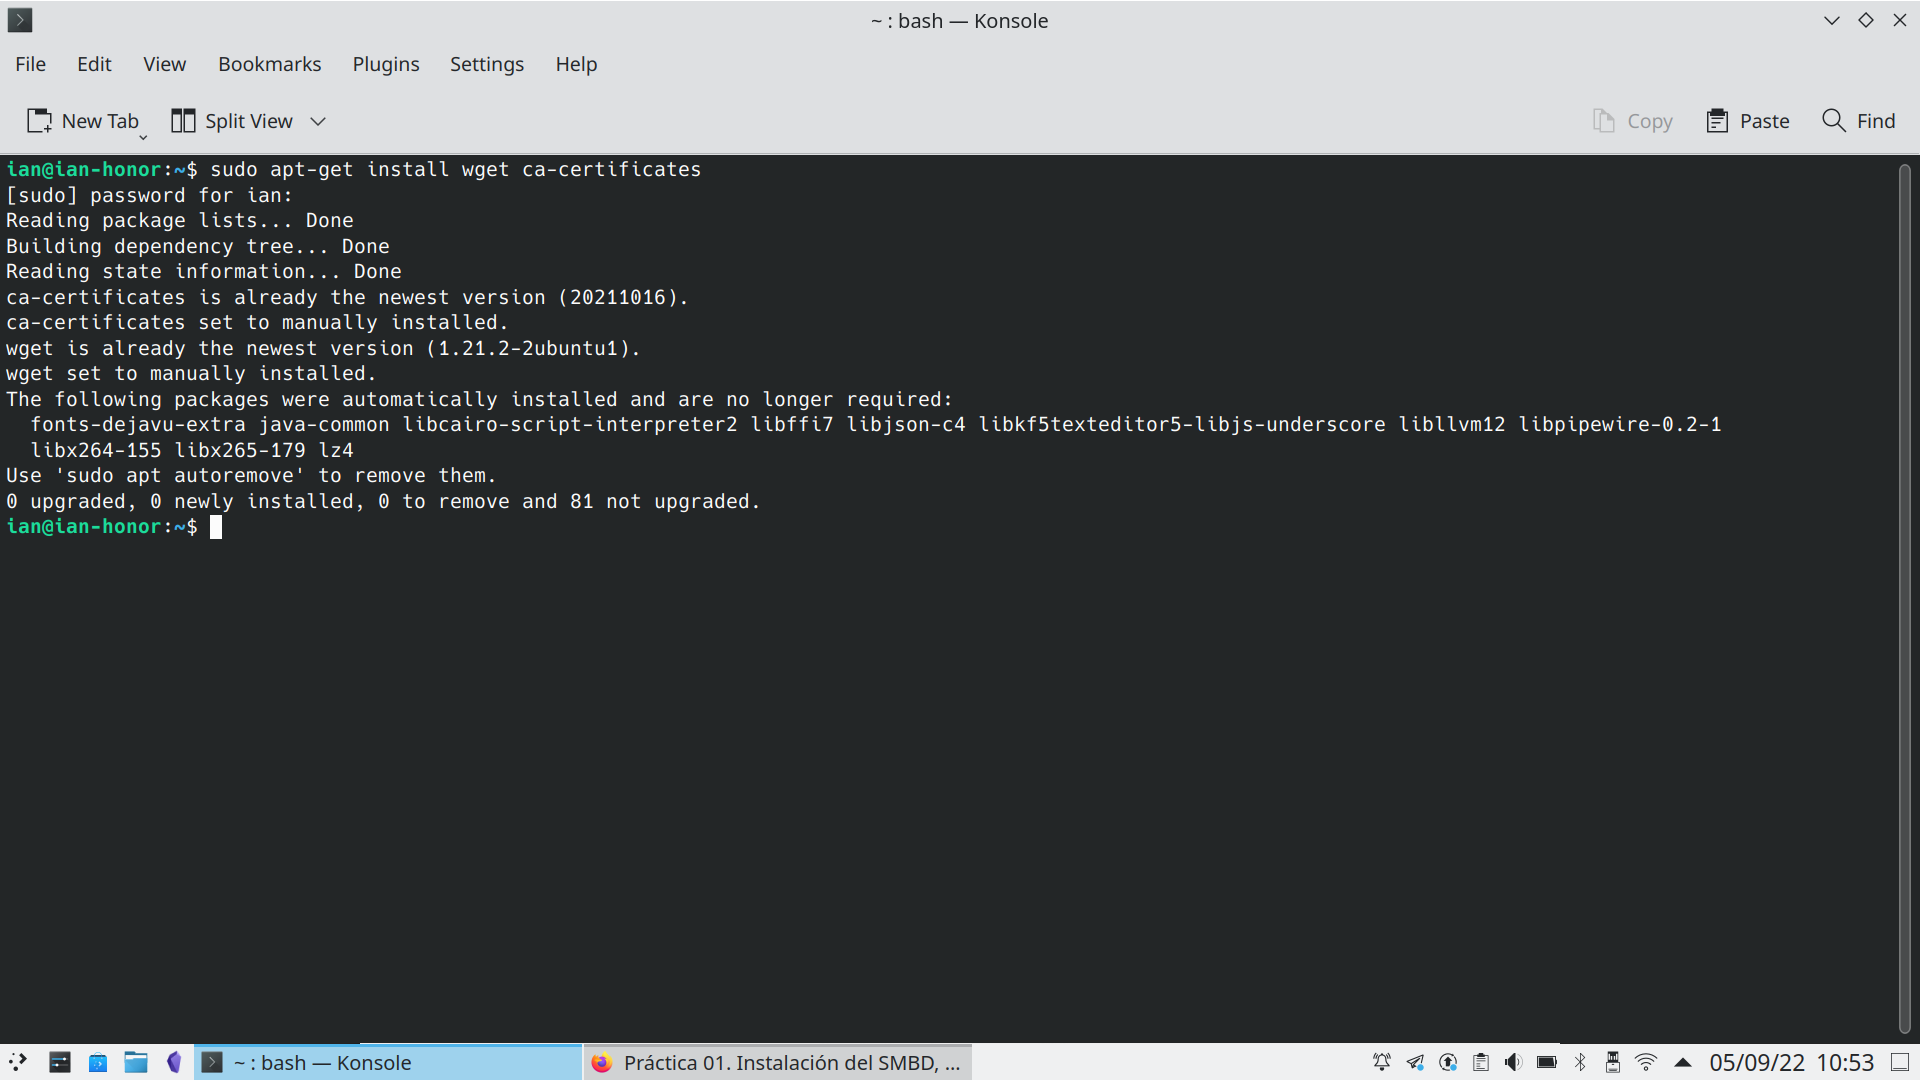
\includegraphics[scale=0.3]{assets/ian_0.png}

        Después, agrego la GPG key de PostgreSQL: \\
        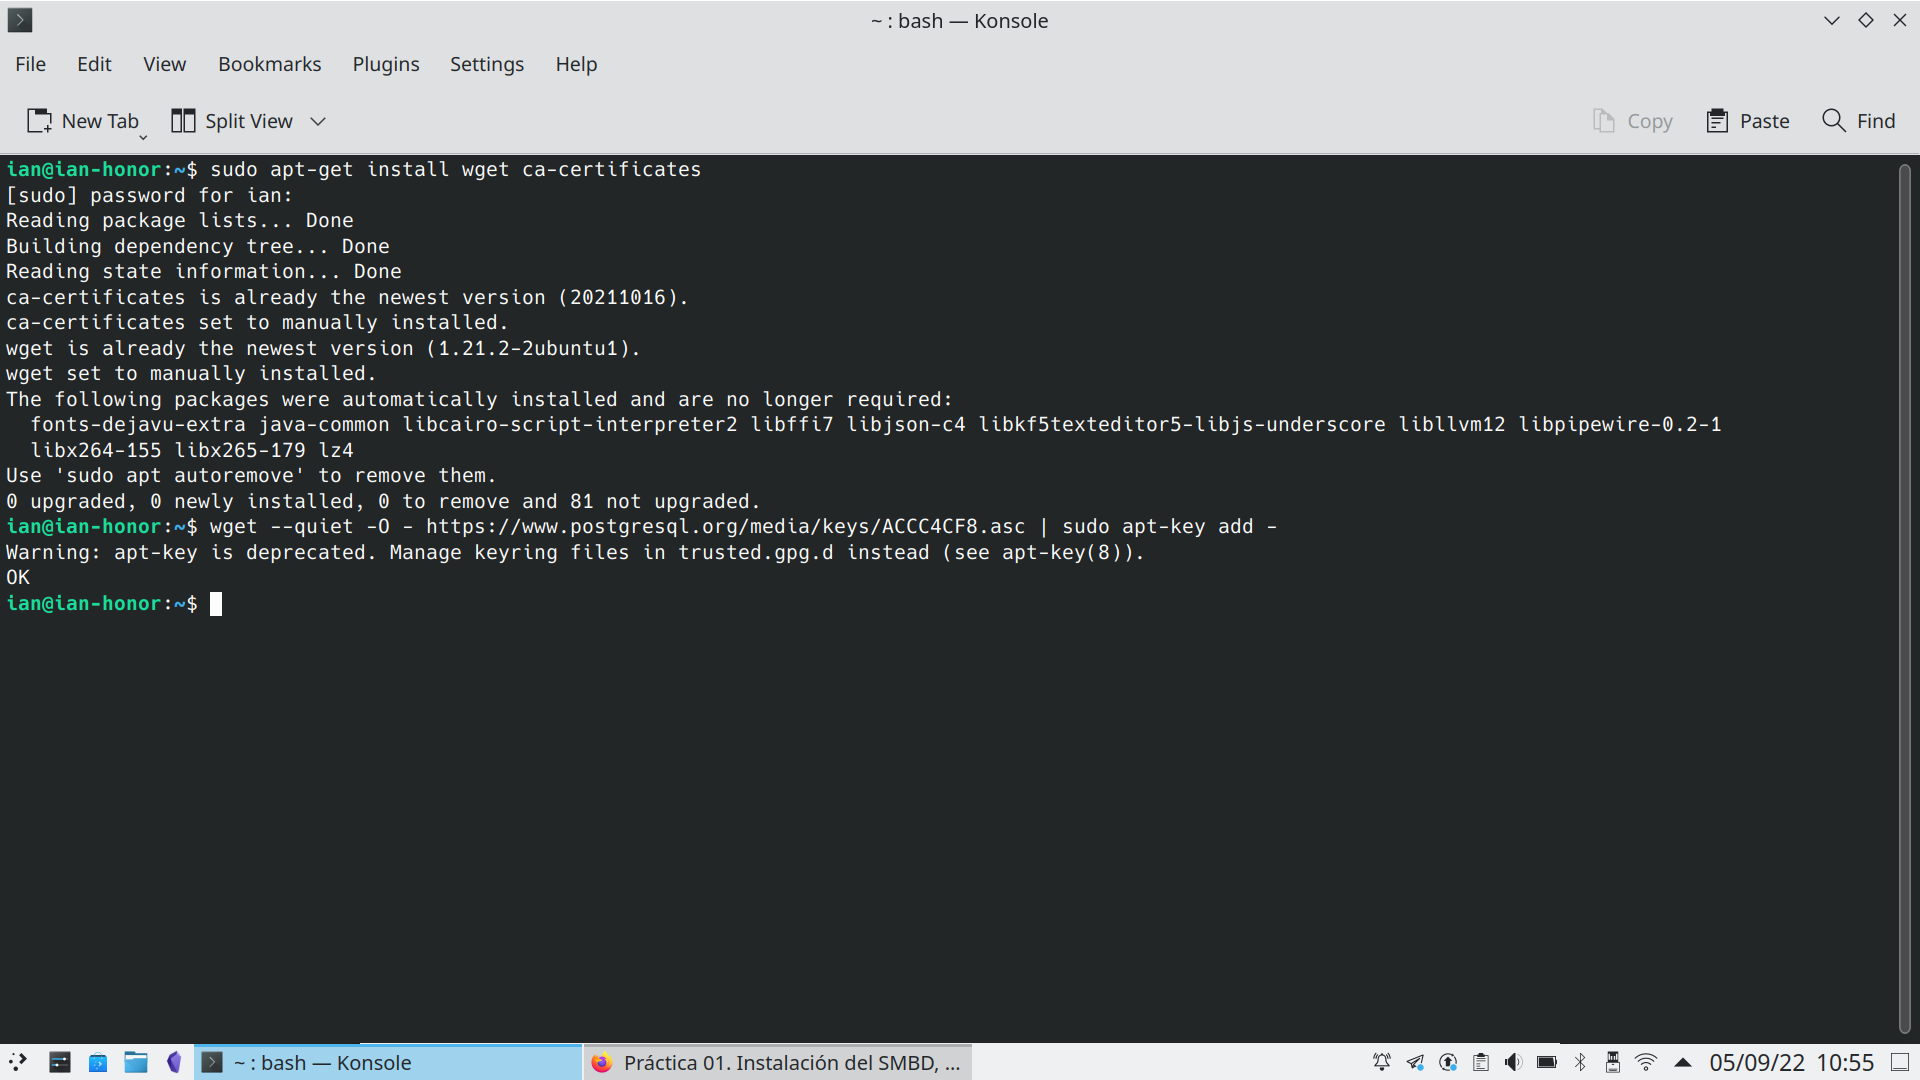
\includegraphics[scale=0.3]{assets/ian_1.png}\\
        
        Posteriormente, intento agregar la GPG key de PgAdmin, momento en el que me doy cuenta que no tengo instalado curl:\\
        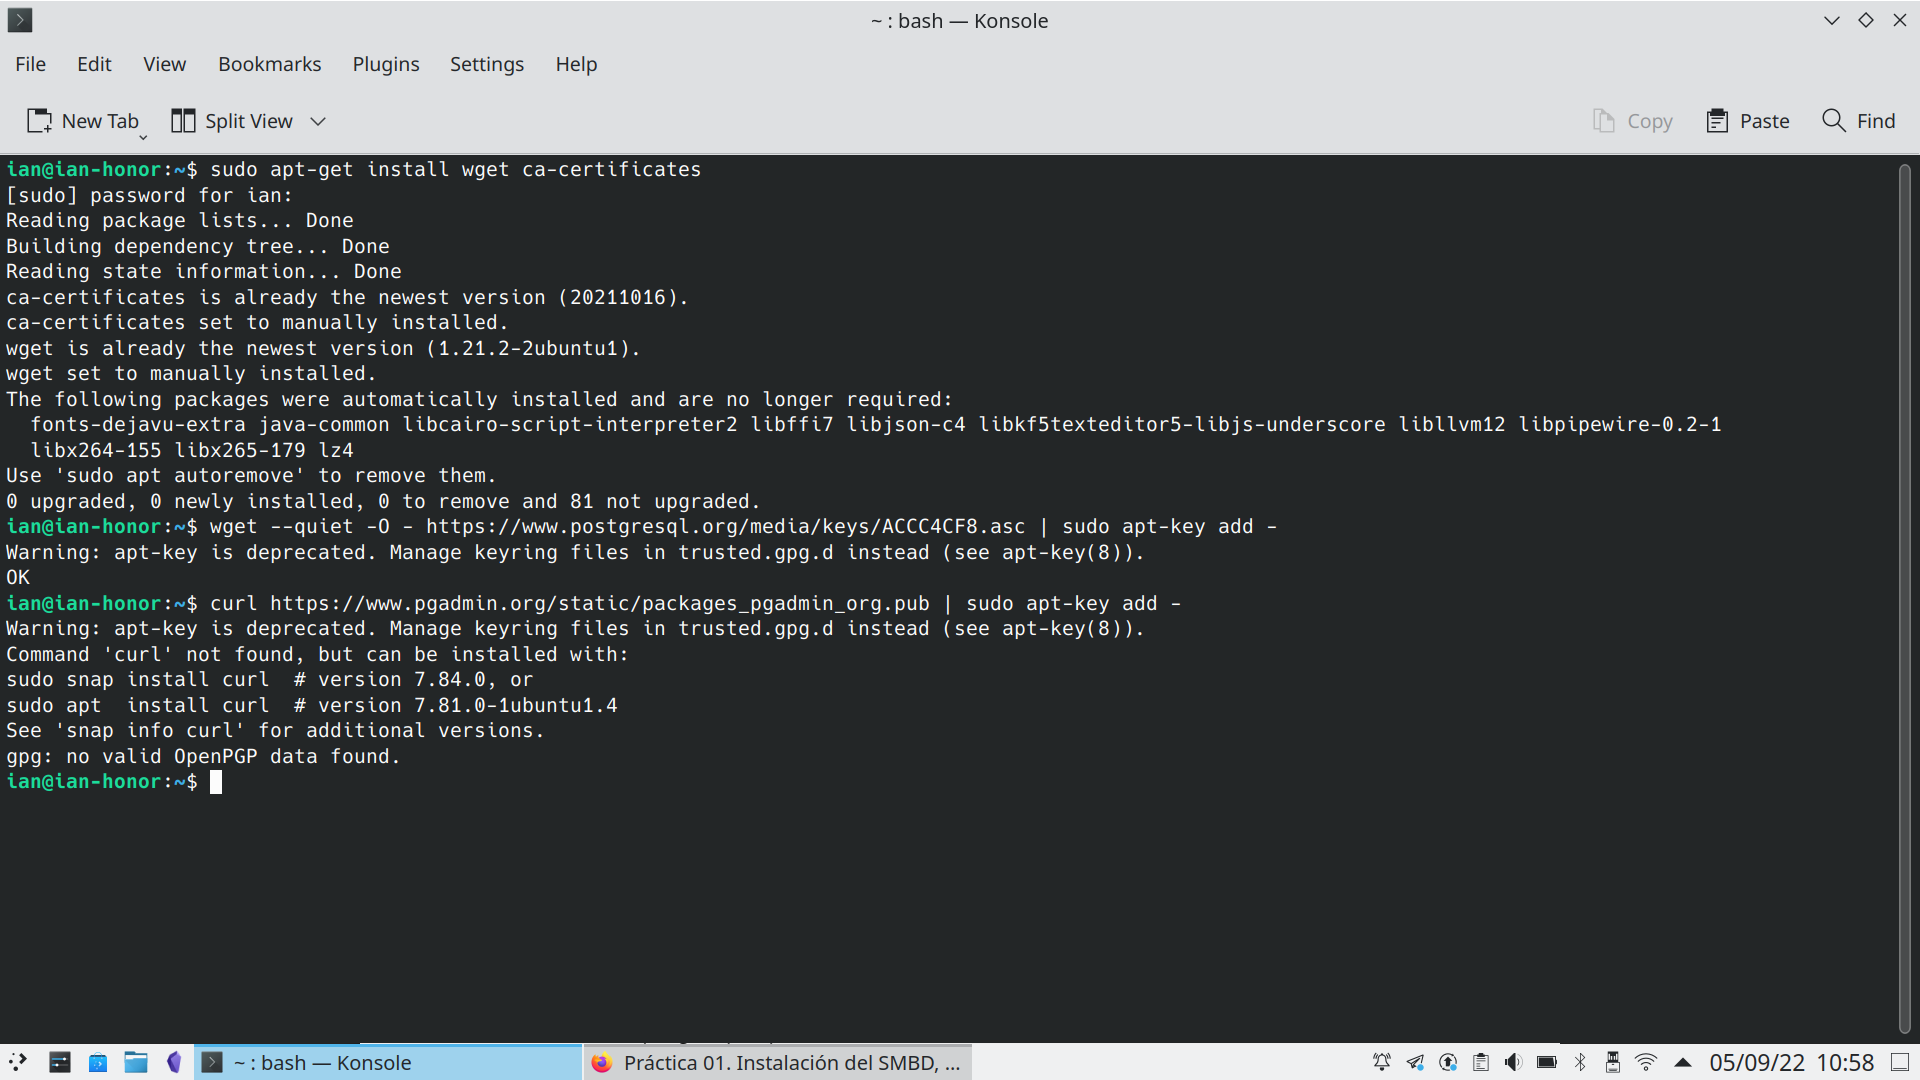
\includegraphics[scale=0.3]{assets/ian_2.png}\\

        Por lo que procedo a instalar curl:\\
        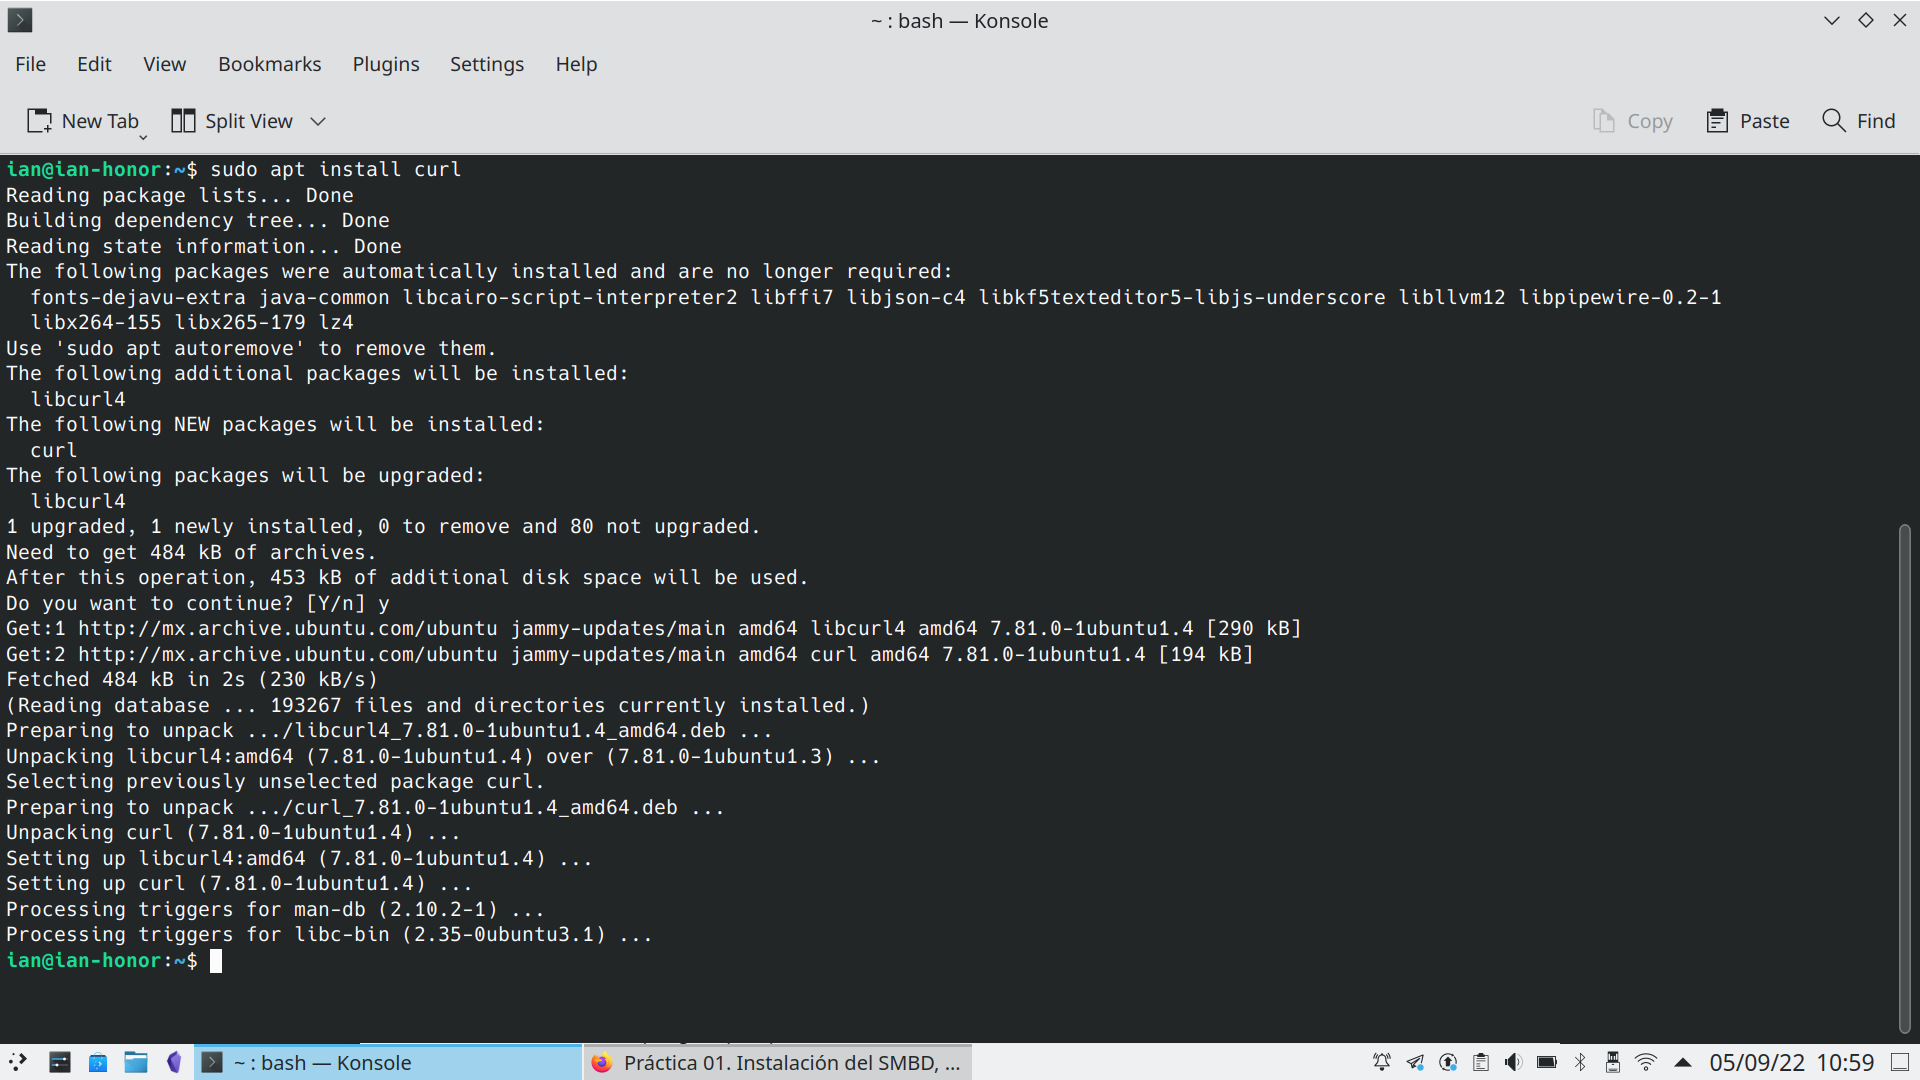
\includegraphics[scale=0.3]{assets/ian_3.png}\\

        Después de lo cual, agrego la GPG key de PgAdmin con normalidad, y procedo a agregar los repositorios oficiales de PostgreSQL y PgAdmin:\\
        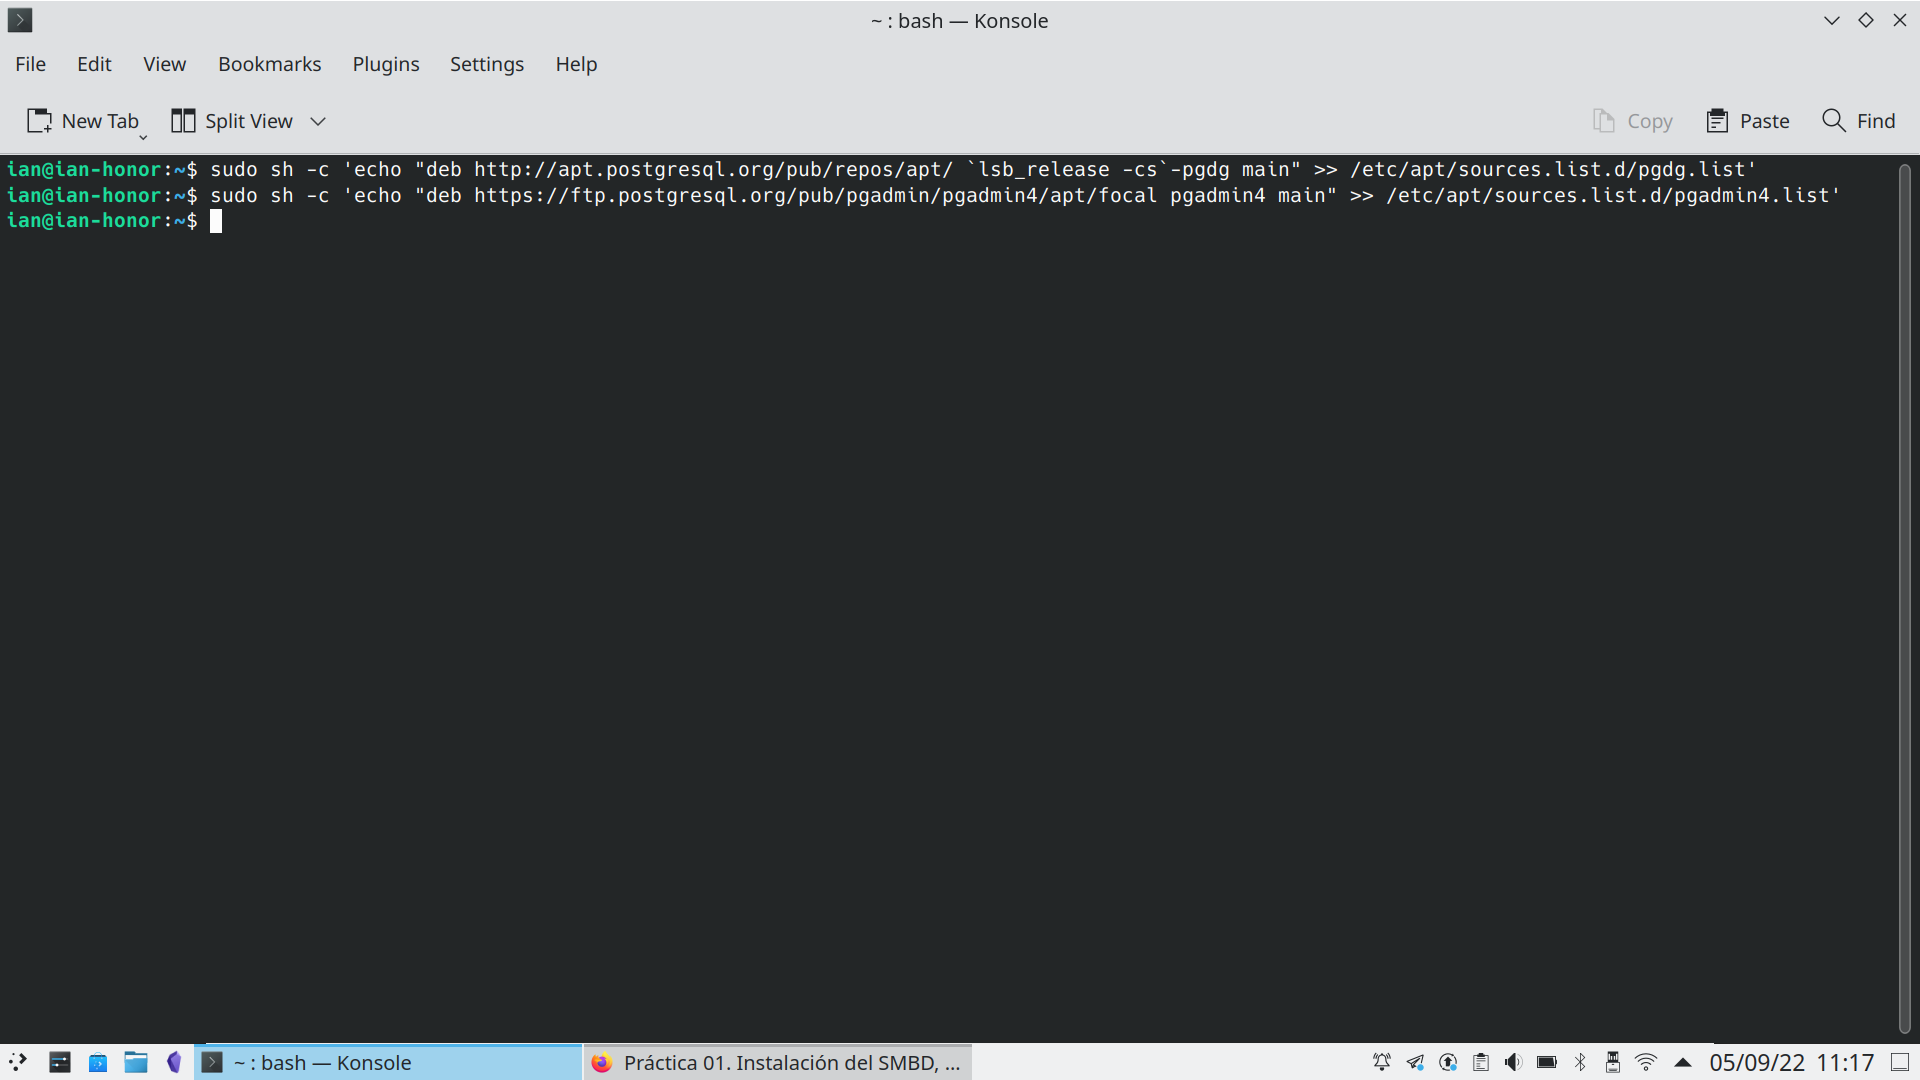
\includegraphics[scale=0.3]{assets/ian_4.png}\\

        Y actualizo la lista de paquetes:\\
        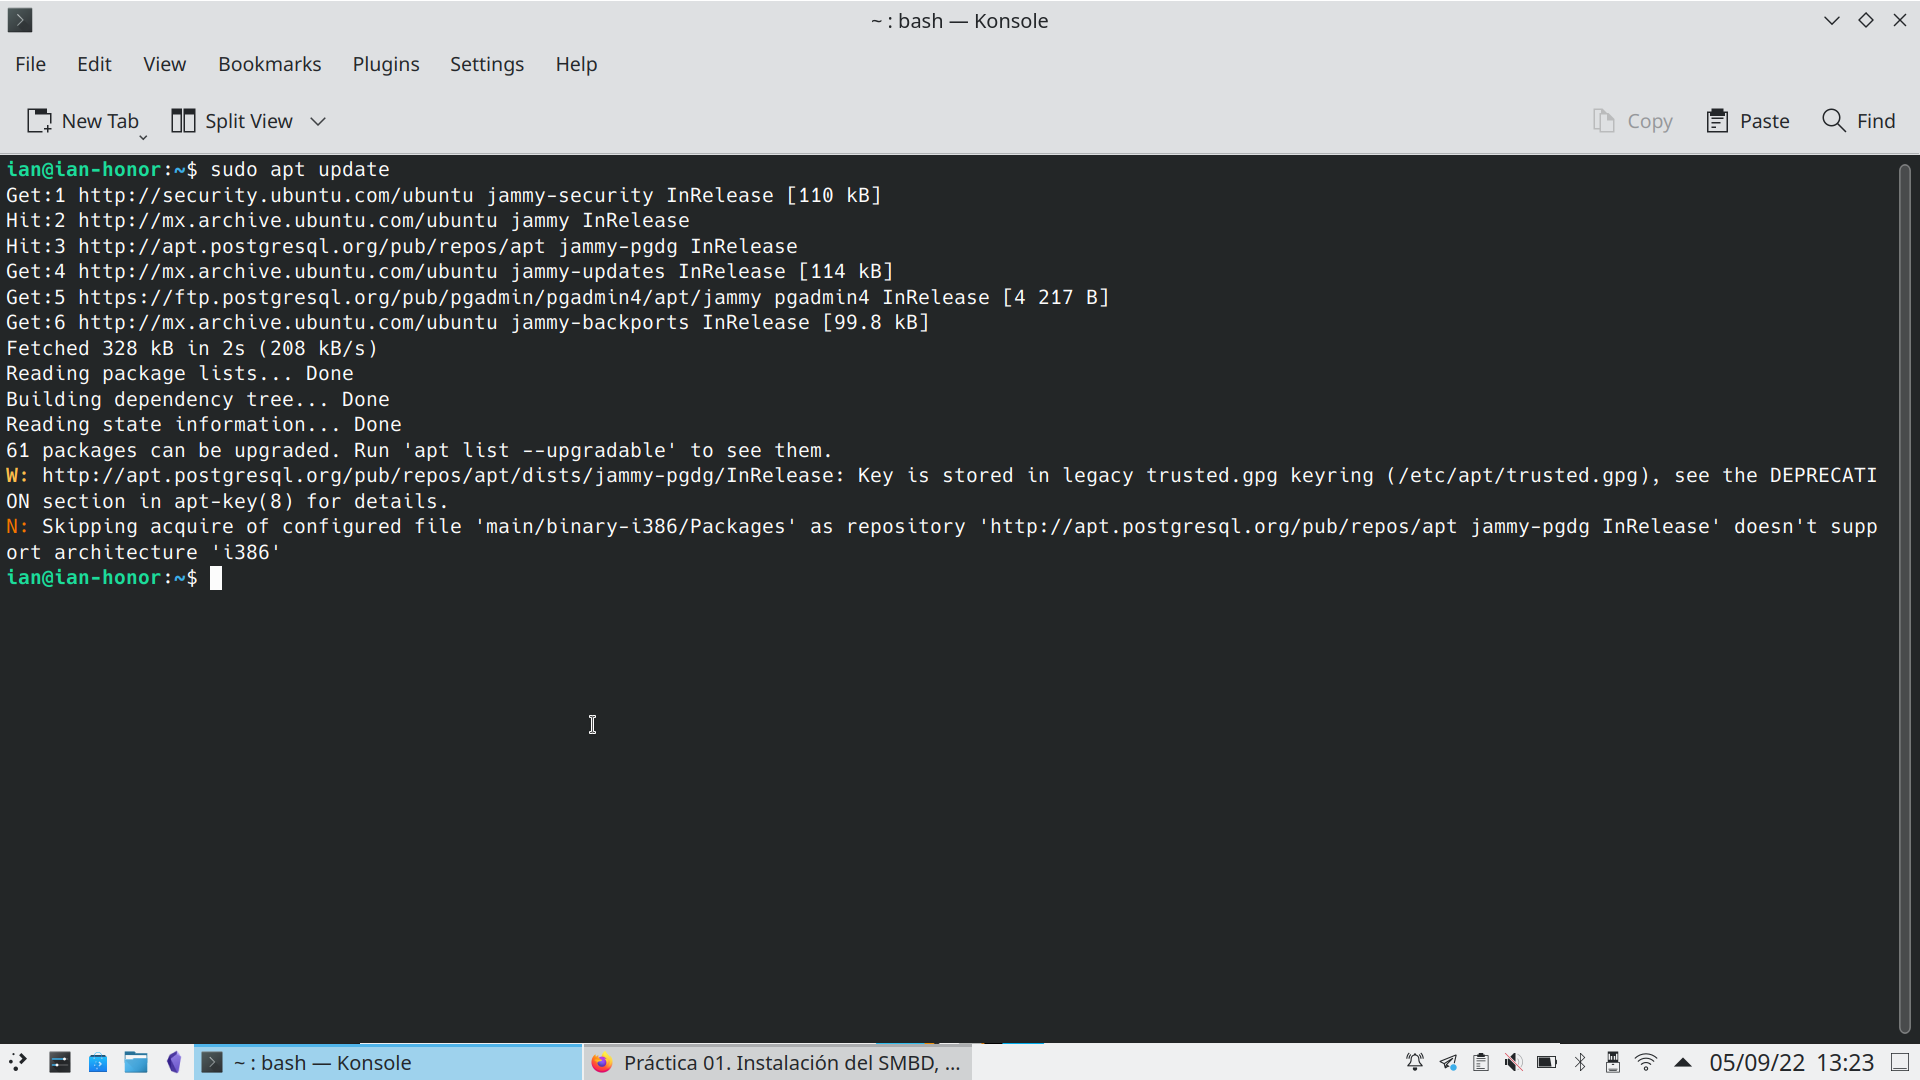
\includegraphics[scale=0.3]{assets/ian_5.png}\\
        
        Con lo cual, finalmente puedo instalar los paquetes:\\
        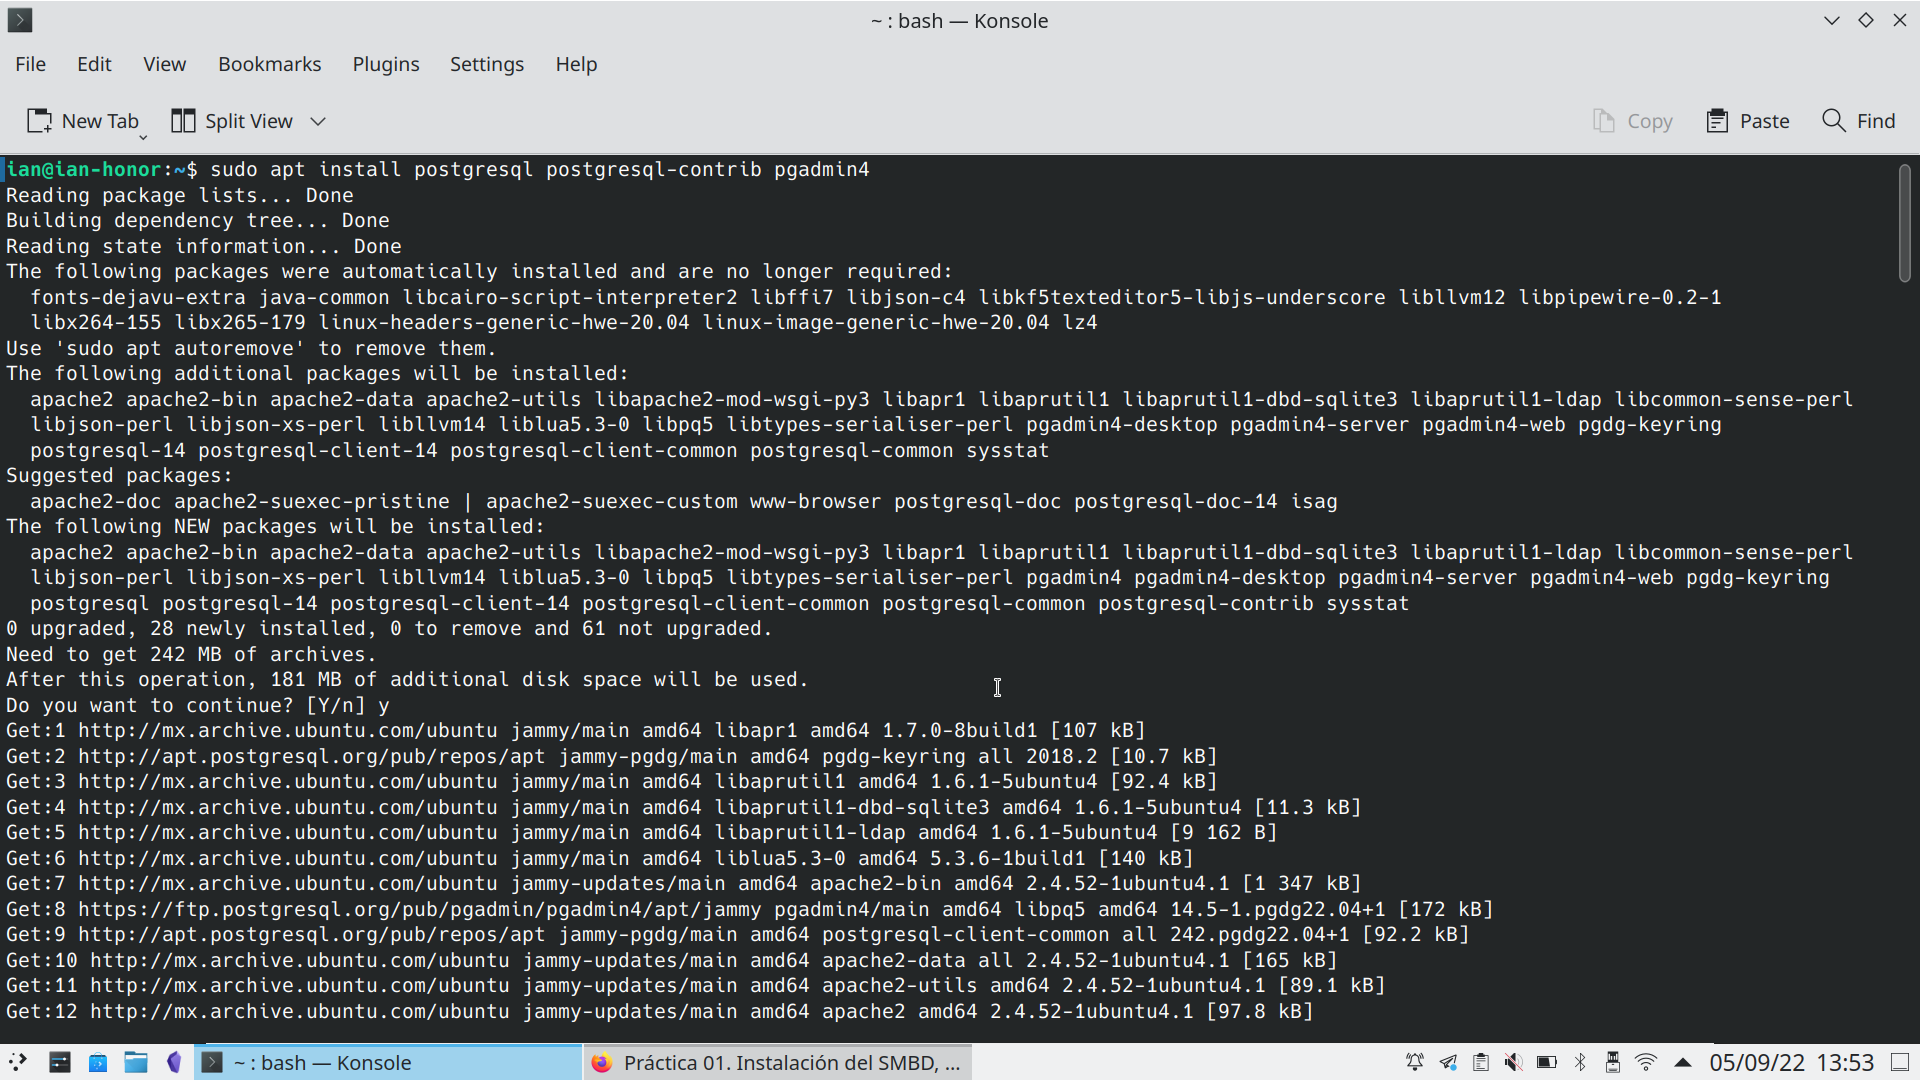
\includegraphics[scale=0.3]{assets/ian_6.png}\\

        Verifico el estado de la instalación:\\
        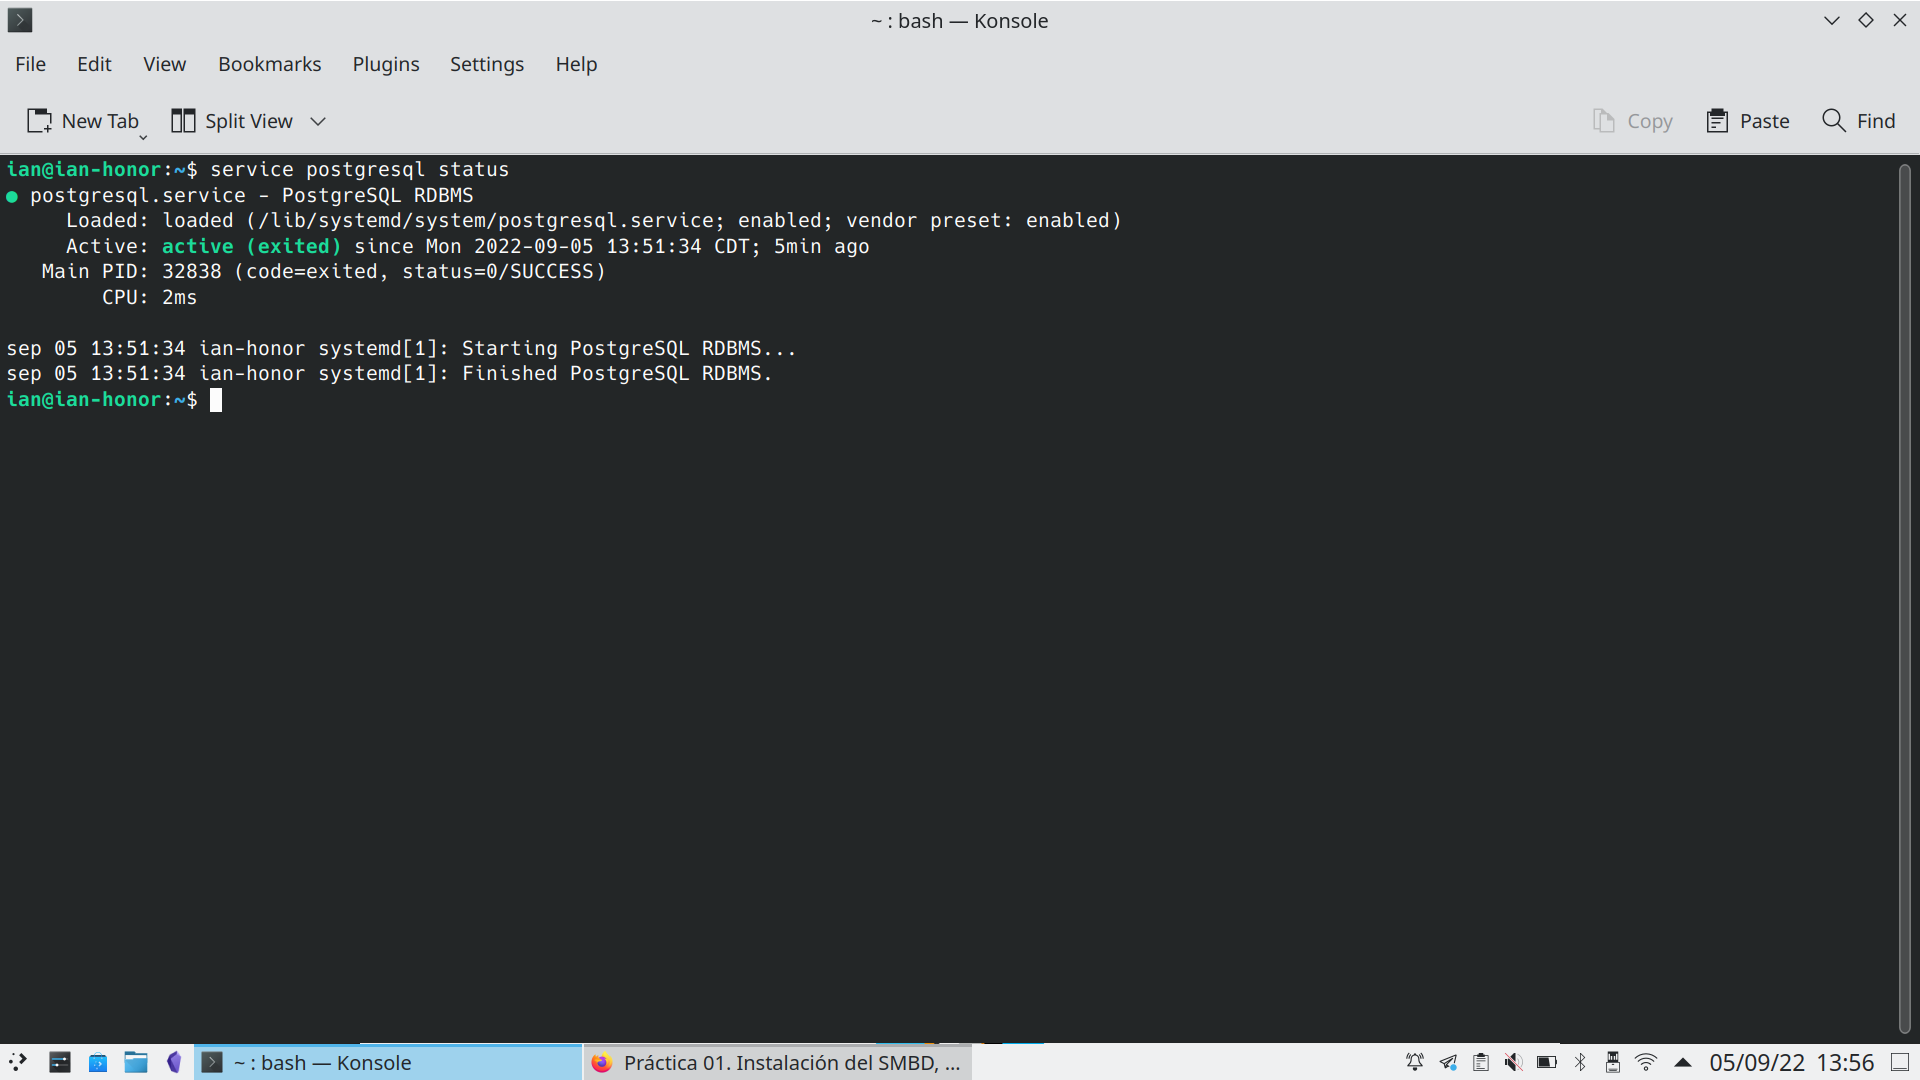
\includegraphics[scale=0.3]{assets/ian_7.png}\\
        
        Habiendo hecho esto, establezco una conexión con la base de datos:\\
        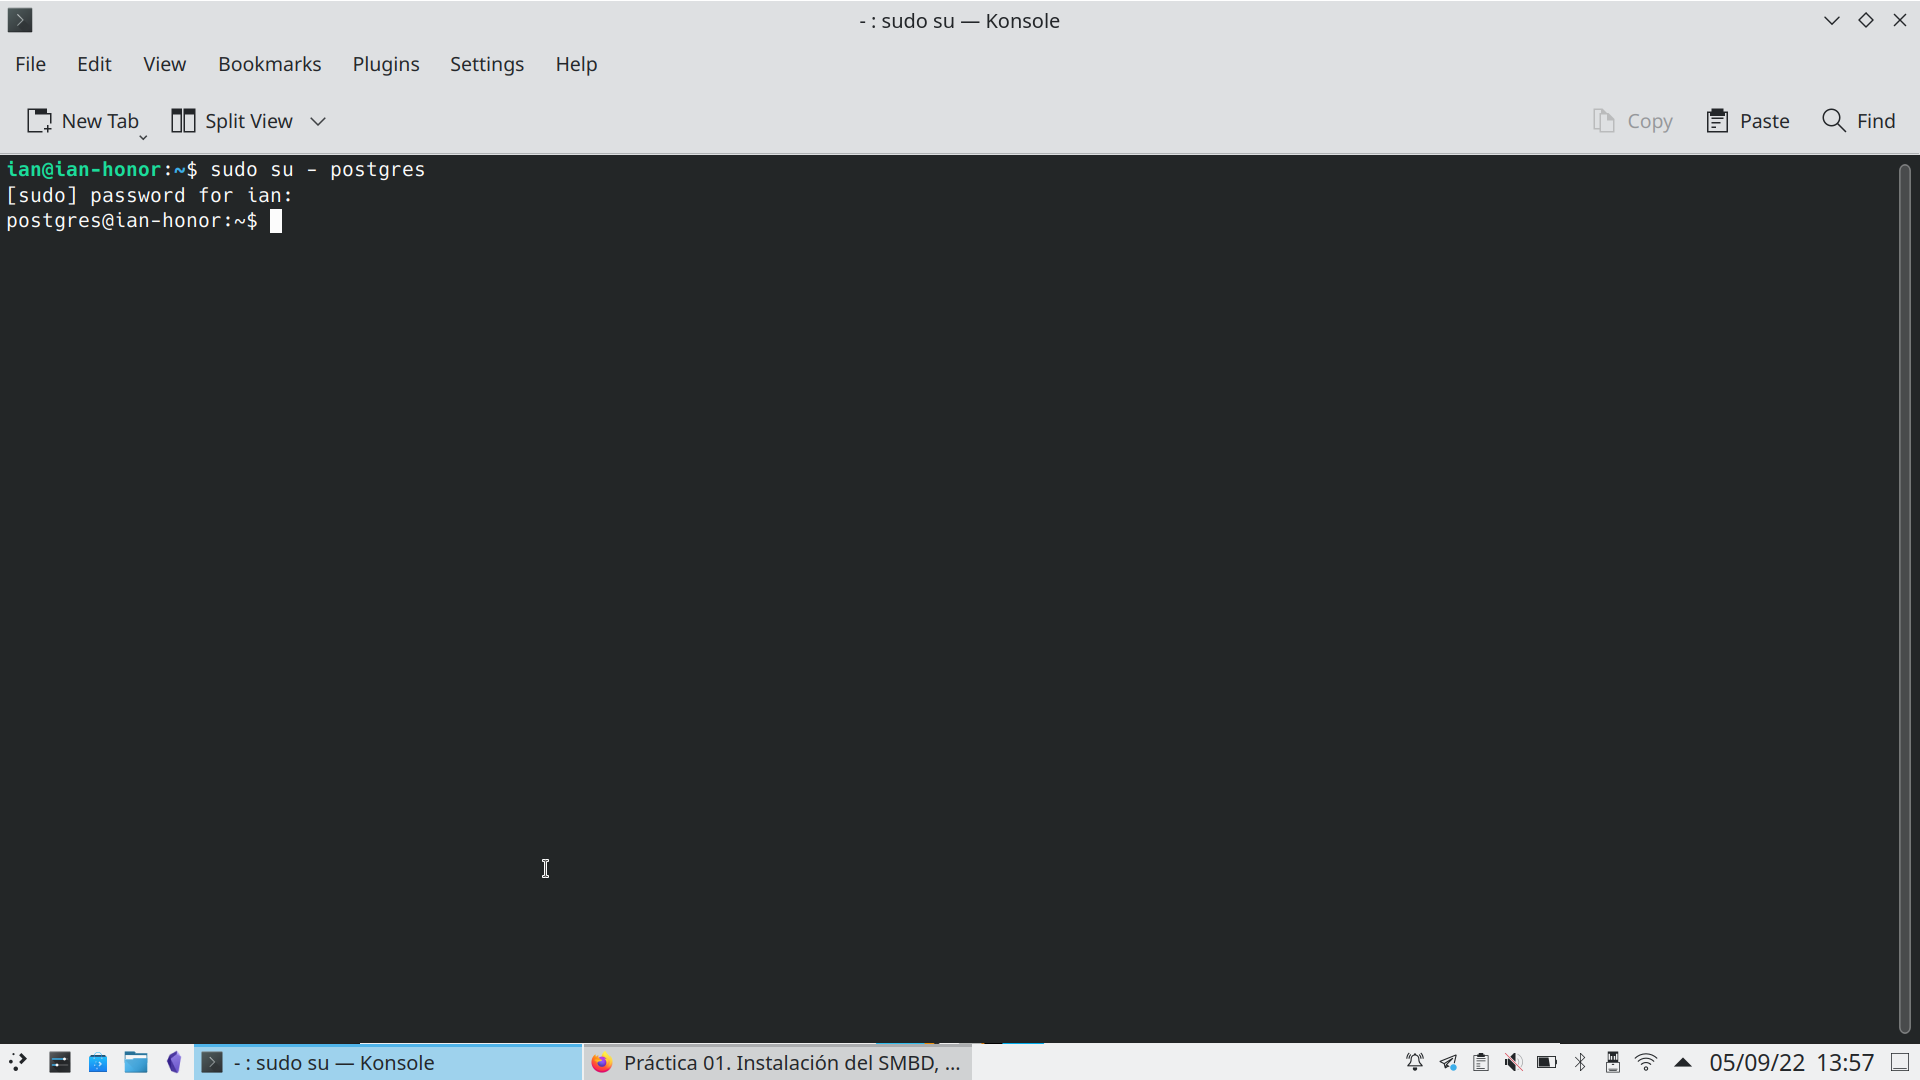
\includegraphics[scale=0.3]{assets/ian_8.png}\\
        
        Y para finalizar, abro el prompt y cambio la contraseña del superusuario:\\
        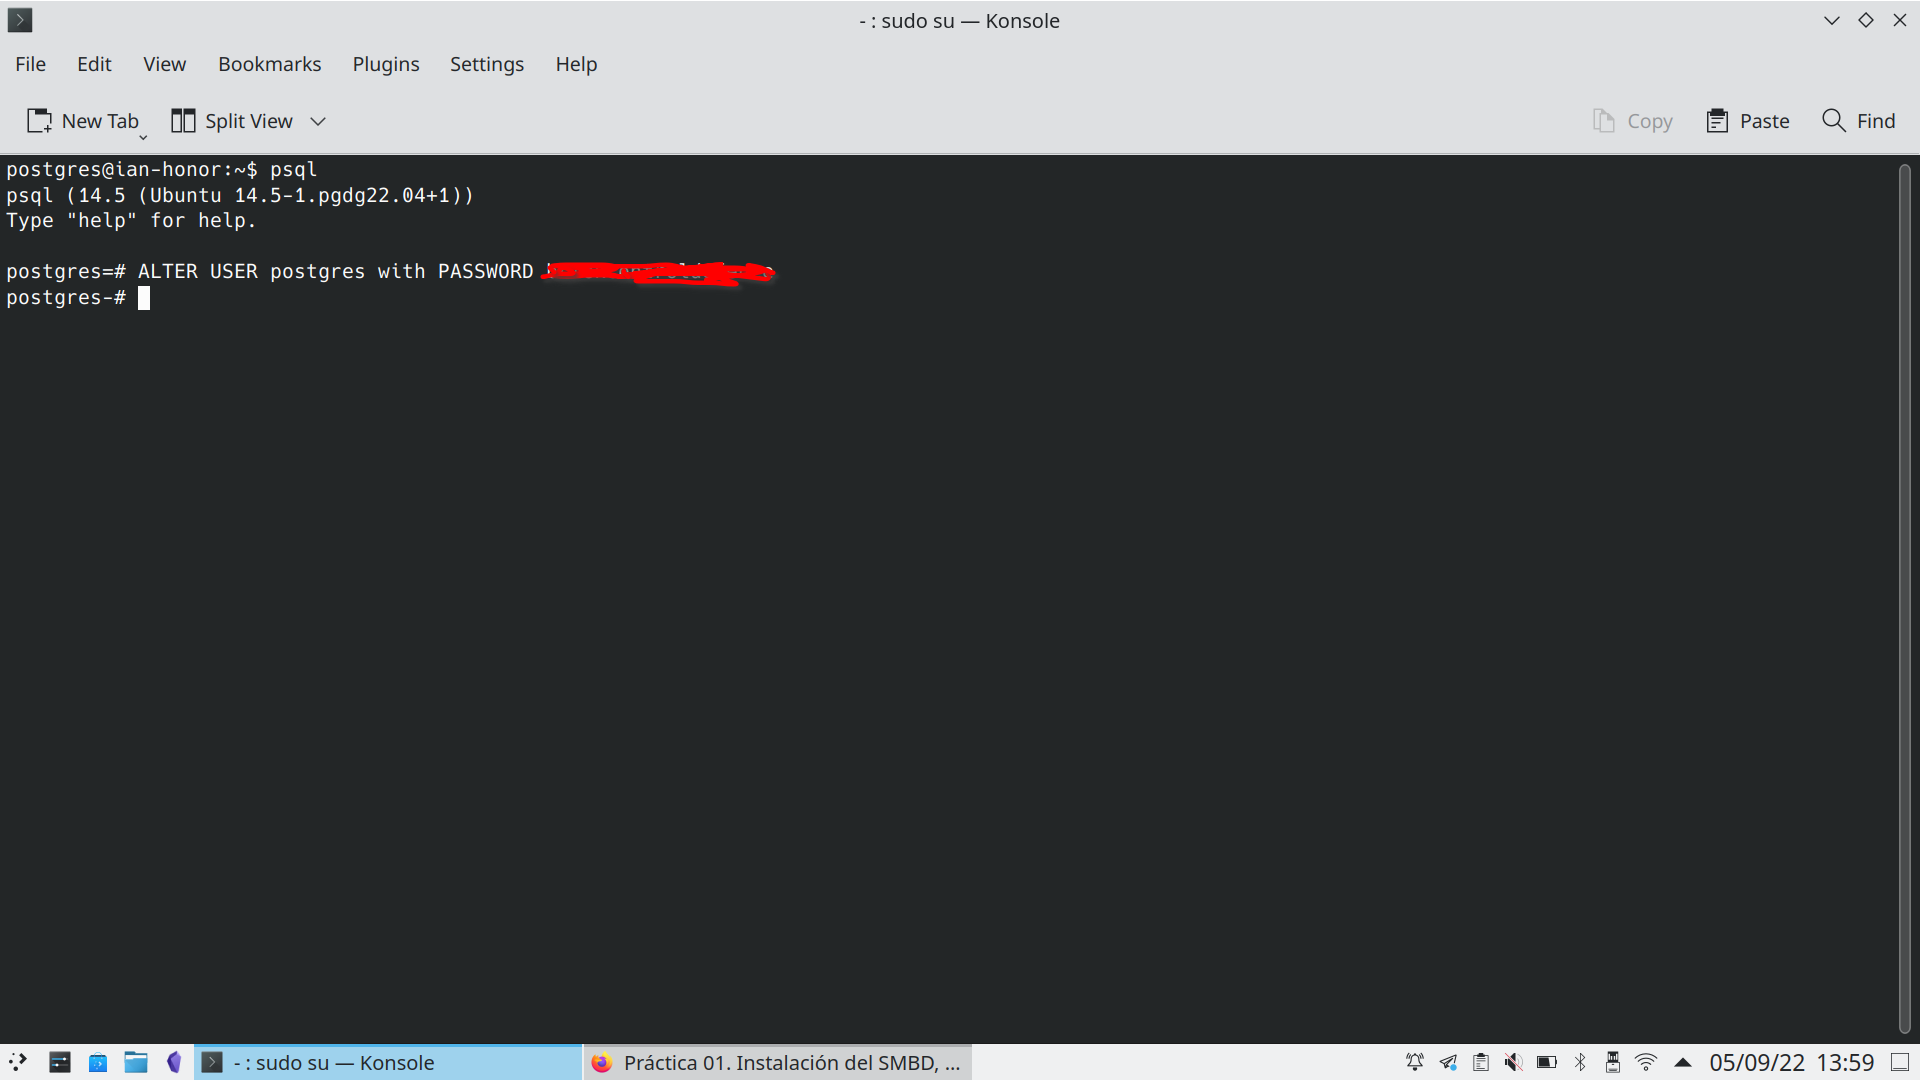
\includegraphics[scale=0.3]{assets/ian_10.png}\\

    \item \textit{Comentarios y problemas:}\\
        Afortunadamente, ya que uso ubuntu, pude seguir todos los pasos del pdf de la práctica, lo cual no fue complicado.

        El único problema con el que me enfrente fue el que no tenía instalado curl, pero instalarlo fue bastante simple.
\end{enumerate}

\end{document}

